\documentclass{article}
\usepackage[utf8]{inputenc}
\usepackage{amsmath}
\usepackage{amssymb}
\usepackage{changepage}
\usepackage{graphicx}
\allowdisplaybreaks
\title{Homework 4 Writeup}
\author{Michael Tang}
\date{due June 14, 2019}
\begin{document}
\maketitle
\begin{adjustwidth}{-2cm}{-2cm}
\section{Usage}
Use ``make'' to compile and link the modules from utils and from the root directory. ``make clean'' is available to remove all .o files. This time, alterations have been made to the utils folder, including the addition of locks.c and locks.h, so it is imperative to have my version of utils in the same parent directory.\\
Execute the program as follows:\\
./pachand [-n \textit{nsrc}] [-W \textit{pkwk}][-M \textit{timelim}][-T \textit{npck}][-D \textit{qdepth}][-A \textit{addpor}][-R \textit{rempor}][-p \textit{pflag}][-h \textit{hitrate}][-H \textit{htable}][-d \textit{remcorr}][-o \textit{outpath}]
\begin{itemize}
	\item -n specifies number of sources. In parallel mode this translates to number of worker threads (so the total number of threads will be n+1). Required.
	\item -W specifies average work per packet. Required.
	\item -M specifies time limit for threads, in milliseconds. All threads will run until the time limit is reached. Due to time difference measurement in-program being based in seconds, -M must be a multiple of 1000. Either this or -T but \textbf{not both} must be specified.
	\item -T specifies number of packets each worker thread is to process. This was used for correctness testing purposes only. This XOR -M must be specified.
	\item -D specifies queue depth, default 8 if not specified.
	\item -A is the ratio of packets that will be add packets.
	\item -R is the ratio of packets that will be remove packets. A and R must not add to more than 1 and must both be positive.
	\item -p is a flag with default value 0. If 0, the program will run in serial mode, if 1, the program will run in parallel mode, and if 2, the program will run in parallel-no-load mode.
	\item -h is the hitrate, the theoretical proportion of contains() calls that would succeed.
	\item -H is the hash table type, 0 for serial, 1 for striped lock, 2 for optimistic striped lock. 0 can only be used for serial operation mode and 1 and 2 can only be used for the parallel operation modes.
	\item -d is a flag with default value 0 which, when set to 1, strictly handles half add packets, then half remove packets, in serial mode. Used for the correctness testing of serial remove outputted in ``remove\_correctness.txt''.
	\item -o is the path for the file to which user wants to output. If not specified, program will default to stdout. \textbf{WARNING:} files open in append mode. If you want to start a clean version of existing output files make sure to remove them first.
\end{itemize} 

\section{Design Changes}
\subsection{Locks and Queue Strategy}
Initially, it was intended for lock type and Lamport Queue strategy to be changeable at the command line. However, HashPacket's uniform checksum distribution meant that even in the Awesome strategy I had implemented in HW3b, dequeueing threads would not be floating between queues that much, and contention on those queue's locks would be removed. This made TASLock the clear choice of lock for Lamport Queues, due to their low memory overhead compared to other locks and nonexistent system call overhead. For the striped lock hash table, I learned via a student's Piazza post about the pthread\_rwlock\_t struct, whose ease of use far outweighed any possible performance boost I might have gotten from crafting my own read-write lock structure.\\
For Lamport Queue strategy, I re-tested my Awesome queue from HW3b with uniform packets, and compared speedup to the lock-free version. The data and graph for this test at $W=4000$, which is the only work level used for this project's performance experiments, are below:\\
\null\\
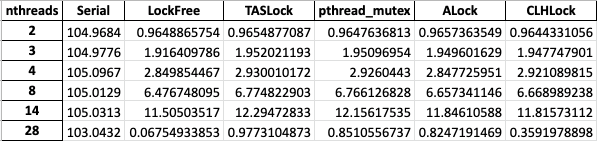
\includegraphics[width=\linewidth]{awesomeq_vs_lockfree_data.png}\\ \null\\
\null\\
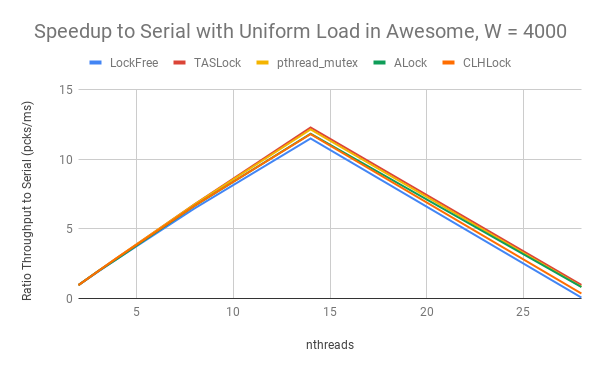
\includegraphics[width=\linewidth]{awesomeq_vs_lockfree_graph.png}\\ \null\\
Observable in this data is a much more reduced performance boost compared to the test with exponential packet distribution, which is reasonable as the main speedup factor of Awesome mode was unequal distribution of work. But since it is a performance boost nevertheless, I opted to set Awesome mode as queue strategy.
\subsection{Hash Table Operation}
Since the versions of hashtable.c and seriallist.c that we received in utils did not account for a case where adding is conducted on a key that is already in the table, I assumed throughout initial development that Add would never be called on an existing key. Only while debugging a resize issue did I notice that duplicate Adds indeed existed. This was especially visible on the parallel versions, where second Adds on an existing key that would maybe have serially come after a Remove operation on that key instead came before, due to concurrency.\\
To accommodate this, I changed the design of seriallist.c : addNoCheck\_list to check for key equivalence when searching across a bucket, and if the key to be added is matched with a key in the bucket, the node in the bucket is updated with the new packet that was supposed to be added.\\
For my Awesome design I picked an optimistic striped-lock hash table, which lets threads calling Contains() first attempt to read without a lock before trying again with a lock if they fail. This involved changing key node change operations in Add, Remove, and Resize to atomic TestAndSets in order to ensure other threads read a valid hash table at all times. However, while struggling with implementing that correctly I realized that the actual state changes that these operations can be linearized on (adding a new node to a bucket in Add, removing a node from a bucket in Remove, and updating the size of the hash table in Resize) did not themselves have to be atomic, as there was no other thread competing to make a change. This significantly improved the ease of implementation, as now the key idea was just to ensure that changes were only visible in the last step. Add and Remove especially benefitted as the existing versions for regular striped lock could be used exactly the same for optimistic.

\section{Testing Results}
\subsection{Correctness}
To keep ensuring Lamport queue correctness, I re-utilized the tests from HW3b that used -T to get a fixed number of packets, and ensure that the total sum of checksums for packets processed were the same as that of dispatched packets. Also like before, total number of packets processed were still checked for equivalence to total number of packets dispatched, and both parallel modes with both sorts of parallel hash tables had their checksum totals compared to serial.\\
To ensure that no packets were unintentionally duplicated or dropped in the hash table, sum of checksums was accumulated from packets added, and that sum compared to the sum of checksums of packets removed and packets still remaining in the table at end of program. 
Tests for the above can be found in the hw4 directory, in the form of shell scripts ``htablecorr'' for serial correctness, ``partablecorr'' for striped-lock correctness, ``opttablecorr'' for optimistic striped-lock correctness, and ``edgeopttablecorr'' for a high-stress testing of optimistic striped-lock. This high-stress testing involves cases of high Contains calls concurring with both high Add calls and high Remove calls (separately), and normal levels. Each test except for ``edgeopttablecorr'' has the same test cases to facilitate verification of matching checksums with the serial version. This verification is contained in ``check\_htables.py'', as well as in ``check\_pnoload.py'' for the parallel-no-load case. Both Python 3.7 scripts are in the hw4/tests directory along with all the test outputs, and output verification files that should be blank except for an encouraging message if everything is correct.\\
To ensure the correctness of the serial Remove, which all Remove operations are based on, a special case where the first half of packets are all Add packets and the second half are all Remove packets is used. Correctness of the Remove operation would entail the hash table being completely blank at the end. The shell script used for this test is ``remcorr'', and the output for that test is ``remove\_correctness.txt''.\\
I could not come up with a way to rigorously test the correctness of Contains calls, but the success of a portion of those calls within a ballpark range of the specified hitrate leads me to believe that their behavior is correct.\\
There were no discrepancies discovered in the existing tests, so we can safely conclude that the program runs correctly.

\subsection{Performance}
All performance tests were performed as directed in the instructions. All trials of all modes in every experiment was repeated 5 times and the statistic averaged across those 5 trials. -M 2000 was picked by recommendation, and also good results from HW3b.\\
All performance test outputs are available in hw4/tests with the prefix ``exp[num]''. An Interactive Python Notebook written on Jupyter is saved as ``exp\_process.ipynb'', and is used for processing the data into table format, which can be seen on ``expdata.xlsx''. Pandas 0.24.2 was used for this processing - for the data to be written correctly to the .xlsx file Pandas 0.24.0 and above must be used. All tests except for Optimistic Overhead were conducted in ``sl4.sh''. Optimistic Overhead tests are contained in ``sl4\_optovr.sh''.
\subsubsection{Dispatcher Rate}
The results for this test are available in ``exp1\_disprt.txt''. From these five trials, the average throughput was 1812.49 packets/ms. Comparatively, the average throughput found in HW2's dispatcher rate experiment across all $n$ except for $n = 28$ was 1792.28 packets/ms. $n=28$ was not included due to more threads than cores forcing the dispatcher to context switch with another thread on the same core, and the dispatcher throughput being critically decreased as a result. So on average, this dispatcher enqueues 22.21 packets more per millisecond than the HW2 dispatcher. This difference should be taken as insignificant enough for the two to be equal, because 1. performance testing for HW2 dispatcher rate had only one trial per thread setting, causing higher variance and 2. there have been no significant changes to the dispatcher itself since HW2.
\subsubsection{Parallel Overhead}
The results for the test are available in ``exp2\_parovr.txt'', and the table and graph of the processed data are below.\\
\null\\
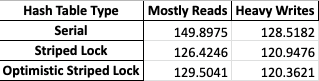
\includegraphics[width=\linewidth]{e2_data.png}\\ \null\\
\null\\
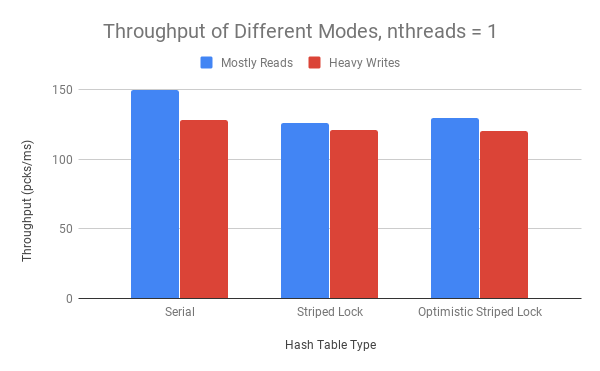
\includegraphics[width=\linewidth]{e2_graph.png}\\ \null\\
The results appear as I expected. The lock-based hash tables have significantly lower throughput than serial in the Mostly Reads load setting (approx. 20 pcks/ms less for optimistic, 23 pcks/ms less for striped-lock), and closer but still lower than serial in the Heavy Writes setting (approx. 8 pcks/ms for both parallel table types). This can be attributed to lack of parallel benefits at this 1-thread setting, and presence of lock initialization and usage overhead. This advantage reduces when Add operation overhead becomes more significant in Heavy Writes.\\
Optimistic striped-lock also has approximately 3 pcks/ms more throughput than regular striped-lock, due to less usage of the lock (0 usage for Contains due to only 1 worker thread operating). This advantage also disappears when writing is a higher concern than reading in Heavy Writes, which is natural as the advantage of optimistic is, again, based on read speedup.
\subsubsection{Optimistic Overhead Over Regular Striped-Lock}
One part of analyzing the tradeoffs of using optimistic striped-lock over regular striped-lock is seeing the overhead of the difference in operations (not including Contains). To this end, I ran the same Parallel Overhead experiment but with $n = 14$ worker threads in order to include performance differences based on lock contention. Usage of the optimistic Contains method was also disabled; so optimistic striped-lock here contains all of the accommodations for a lock-free Contains call, but does not actually use that lock-free call. The results are available in ``optovr.txt'', and below is the processed data and graph.\\
\null\\
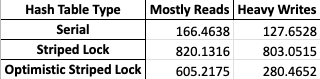
\includegraphics[width=\linewidth]{oo_data.png}\\ \null\\
\null\\
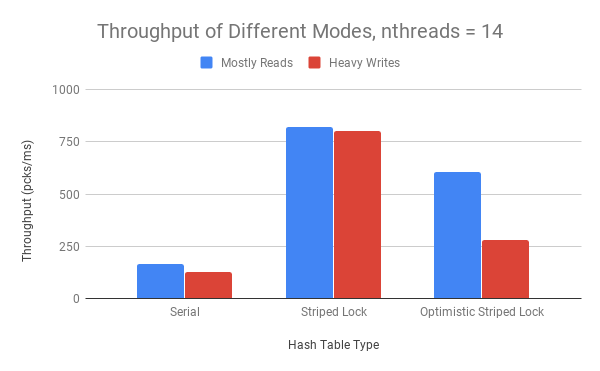
\includegraphics[width=\linewidth]{oo_graph.png}\\ \null\\
Optimistic suffers a reduction of throughput by approximately 215 pcks/ms from regular striped-lock with Mostly Reads load, and a much heavier reduction by approx. 523 pcks/ms from regular with Heavy Writes load. This is expected, as the only difference between the two modes is in handling of resizing. The regular striped-lock mode simply creates a new array of SerialLists and moves the nodes on the existing array of SerialLists to the new one. In optimistic striped-lock, in order to make the visible change to the hash table happen in only one step, an entirely new StripedLockHashTable has to be allocated, new versions of StripedLockHashTable's characteristics have to be allocated and set, and instead of simply being moved the Item\_t nodes have to be copied (via malloc'ing and setting) to the new StripedLockHashTable. Finally, after the one step that swaps the new and old StripedLockHashTables, the old one and its characteristics have to be freed. This is a significant amount of memory overhead that makes optimistic's resizing much slower, as is evidenced when resizings need to be performed more often in the Heavy Writes load setting.\\
The serial data is not actually relevant here, it remains because I copied the SLURM batch file of the Parallel Overhead test and forgot to remove serial tests. It can be taken as a first indicator of how parallel modes can improve over serial.
\subsubsection{Speedup}
The results for this test are available in ``exp3\_spdup.txt''. Following are the results with Mostly Reads load and various hitrates, and analysis at the end.\\
\underline{\textbf{Mostly Reads, $h=0.5$}}\\
\null\\
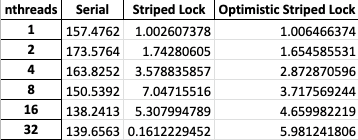
\includegraphics[width=\linewidth]{e3_09_5_data.png}\\ \null\\
\null\\
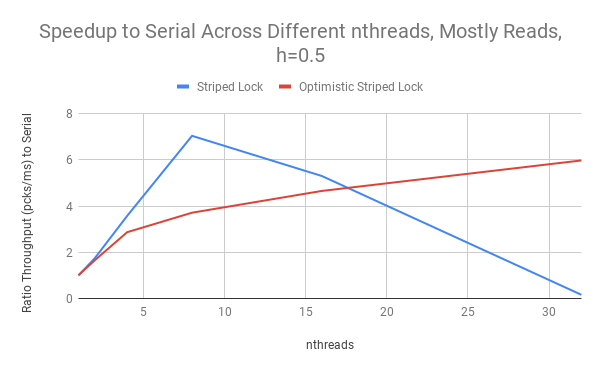
\includegraphics[width=\linewidth]{e3_09_5_graph.png}\\ \null\\
\underline{\textbf{Mostly Reads, $h=0.75$}}\\
\null\\
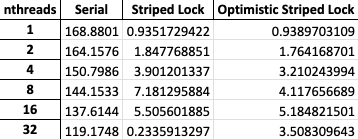
\includegraphics[width=\linewidth]{e3_09_75_data.png}\\ \null\\
\null\\
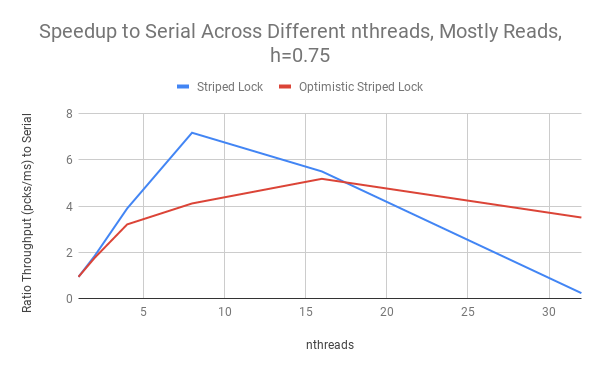
\includegraphics[width=\linewidth]{e3_09_75_graph.png}\\ \null\\
\underline{\textbf{Mostly Reads, $h=0.9$}}\\
\null\\
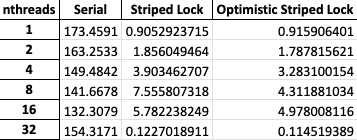
\includegraphics[width=\linewidth]{e3_09_9_data.png}\\ \null\\
\null\\
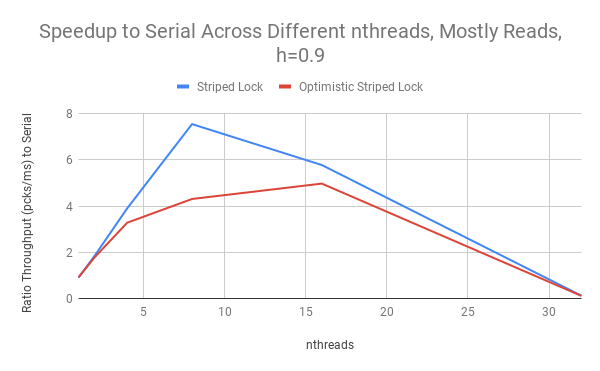
\includegraphics[width=\linewidth]{e3_09_9_graph.png}\\ \null\\
\underline{\textbf{Mostly Reads, $h=0.99$}}\\
\null\\
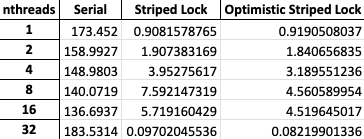
\includegraphics[width=\linewidth]{e3_09_99_data.png}\\ \null\\
\null\\
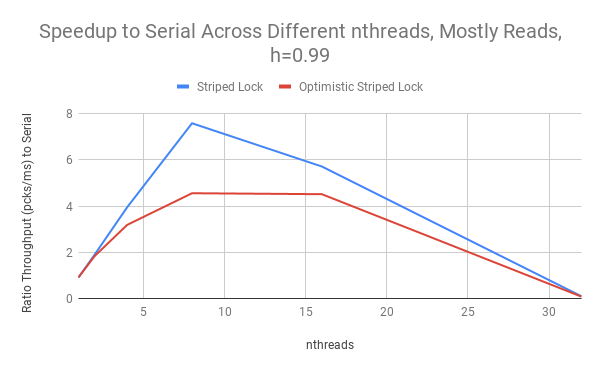
\includegraphics[width=\linewidth]{e3_09_99_graph.png}\\ \null\\
I expected that hitrate would not have much of an impact on the regular striped-lock hash table, and I was correct at least in Mostly Reads load; the data for regular across all hitrates here is practically identical. However, the additional expectation that speedup would remain approximately 1-to-1 linear up to 14 threads was not matched; it was only linear up to 8 threads. What seems most probable is that as the number of threads increased, adds to the same bucket were made more frequently and resizes demanded more. Then, past 8 threads, the amount of additional packets processable were critically outweighed by this resize cost, slowing the operation. This downward trend continues in its own fairly linear motion.\\
For optimistic, I expected increase in speedup to be more than for regular due to the higher proportion of reads, and to also be more stable at $n>14$ threads due to less need for lock usage and therefore less blocking of threads trying to read. I also expected that higher hitrate would increase the performance of the optimistic striped-lock hash table, because I reasoned that more successful Contains calls should mean that optimistic should fail less on the first, lock-free try and thus save time. However, the results did not support a lot of this; the only really correct expectation was the stability one. Increase in speedup was lesser sloped than for regular (2x from $n=4$ to $n=8$ in regular versus 1.33x in optimistic), likely due to the much more costly resize operation. The ability of optimistic Contains calls to try surpassing costly blocking from writes did shine at $n>8$, as optimistic did not experience the same collapse in speedup as regular there. An almost completely contrary result came regarding effect of higher hitrate;  at $n=14$ threads and below the throughput data remained practically identical across all hitrates, while at $n>14$ the speedup went from stable increase at $h=0.5$ to a decrease just as sharp as the regular's at $h>0.9$. A review of my code does not bring forth any potential for this contrary behavior, so I believe that this behavior stems from the nature of the HashPacket generator. Likely is that, to fulfill this higher hitrate, the generator outputs the write packets more towards the beginning, to the point where at $h>0.9$, to ensure hitrate is practically 100\%, all of the write operations happen first. This leaves much less time for the Contains calls to even happen, rendering the behavior practically identical between optimistic and regular since the only source of speedup for optimistic is barely utilized.\\
\underline{\textbf{Heavy Writes, $h=0.5$}}\\
\null\\
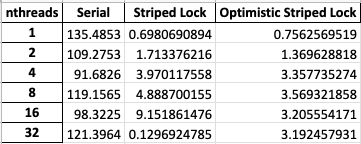
\includegraphics[width=\linewidth]{e3_45_5_data.png}\\ \null\\
\null\\
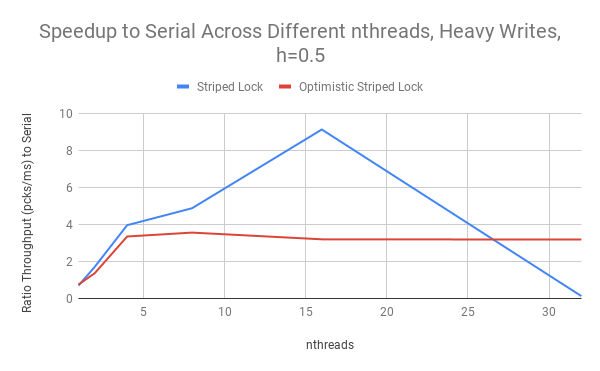
\includegraphics[width=\linewidth]{e3_45_5_graph.png}\\ \null\\
\underline{\textbf{Heavy Writes, $h=0.75$}}\\
\null\\
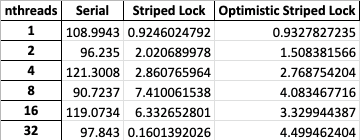
\includegraphics[width=\linewidth]{e3_45_75_data.png}\\ \null\\
\null\\
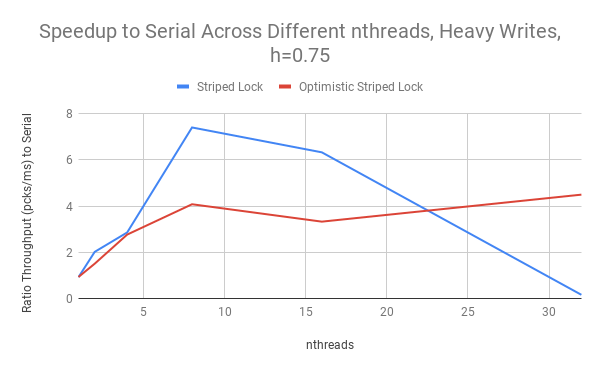
\includegraphics[width=\linewidth]{e3_45_75_graph.png}\\ \null\\
\underline{\textbf{Heavy Writes, $h=0.9$}}\\
\null\\
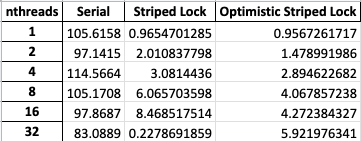
\includegraphics[width=\linewidth]{e3_45_9_data.png}\\ \null\\
\null\\
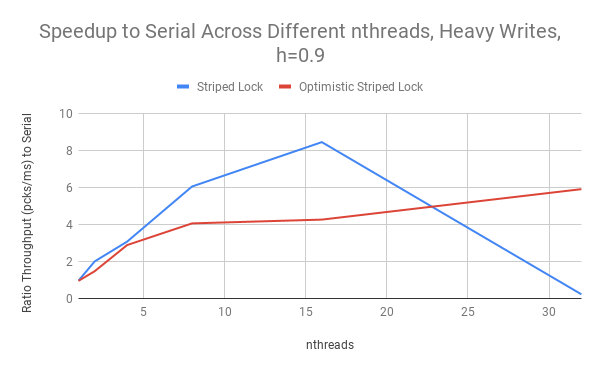
\includegraphics[width=\linewidth]{e3_45_9_graph.png}\\ \null\\
\underline{\textbf{Heavy Writes, $h=0.99$}}\\
\null\\
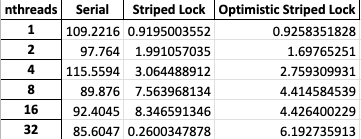
\includegraphics[width=\linewidth]{e3_45_99_data.png}\\ \null\\
\null\\
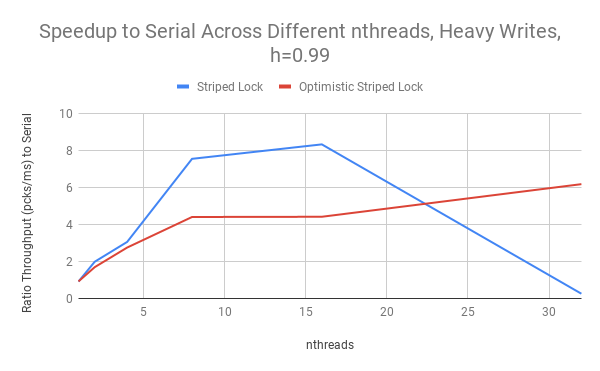
\includegraphics[width=\linewidth]{e3_45_99_graph.png}\\ \null\\
For regular striped-lock here, speedup was worse than linear for lower hitrates but did not experience the same critical decline as in Mostly Reads load. Extending my postulation of hitrate satisfaction behavior from Mostly Reads, this is likely because the higher amount of Add calls forces multiple resize calls to happen earlier instead of over a more extended period of time. Since the significant cost of resizing in regular is its all-encompassing block on other threads, the blocking being less distributed means that this critical loss of productivity in other threads happens less often. Following this behavior postulation, higher hitrates force more adds even earlier and more resize calls earlier, which can explain the better speedup increase at $h>0.75$ from $n=1$ to $n=8$ as additional adds brought by additional threads would not have to force resize if they mostly happen early on. And, the reason for speedup at $8<n<14$ decreasing at $h=0.75$ and increasing for $h>0.75$ could be that for $h=0.75$, even more Add packets brought by more than 8 threads forces additional resizes that did not already happen, while for $h=0.9, 0.99$ most of those resizes already happened at the beginning and no more are needed.\\
Collapse in speedup at $n>14$ threads, like in Mostly Reads load, is likely because additional packets processable is outweighed by higher resize distribution caused by more concurrency.\\
For optimistic striped-lock, the increase in speedup is lesser sloped than in regular but maintains approximately stable increase across all hitrates. In fact, speedup increases more for high number of threads at $h>0.75$, ending at 1.33x the speedup of $h\leq0.75$ at $n=28$. This more closely follows my initial expectation of optimistic performance increasing with higher hitrate, because here the additional resizes are more negligible compared to the resizes already done, and their overhead is trumped by the speedup of more initial lock-free Contains successes.\\
\null\\
A definite conclusion from this experiment is that at lower numbers of threads optimistic is not worth using over regular striped-lock. To improve this outlook, the number of new memory allocations in optimal Resize must be significantly reduced, while still maintaining that the only step visible to other threads is the last step.
\end{adjustwidth}
\end{document}
